\documentclass[lecture.tex]{subfiles}

\begin{document}


\subsubsection{Objectifs du TP}

L'objectif de ce TP est de :
\begin{itemize}[label =\ding{110}, font =\tiny ]
\item Vérifier la formule de la flèche ;
\item Déterminer expérimentalement les modules d'Young des matériaux considérés.
%\item Valider les résultats expérimentaux avec le logiciel RDM 6.
\end{itemize}

\subsubsection{Dispositif expérimental}
Le matériel à utiliser est présenté Fig~\ref{Fig_BancFlex}. Il ne faudra pas dépasser une charge de $20\,N$ sur les poutres.
\begin{figure}[h!]
\centering
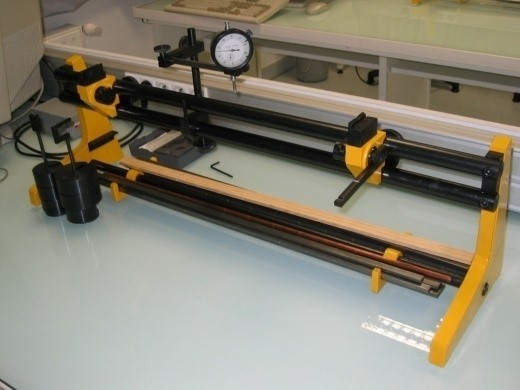
\includegraphics[scale=1]{Img_BancFlexion.jpg}
\caption{Banc de flexion et torsion DELTALAB SAN400.}
\label{Fig_BancFlex}
\end{figure}
Avec ce dispositif expérimental, différentes poutres ou éprouvettes sont fournies dont vous mesurerez les caractéristiques (largeur, hauteur, diamètre) soigneusement au pied à coulisse.

\subsubsection{Essais de flexion}

\paragraph*{Rappels théoriques}
Prenons une poutre de longueur $L$ et de section constante telle que représentée Fig.~\ref{Fig_RDM_Notations}, posée sur deux appuis distant de $d$ et qui serait rectiligne si elle n'était soumise à aucune force.
\begin{figure}[h!]
\centering
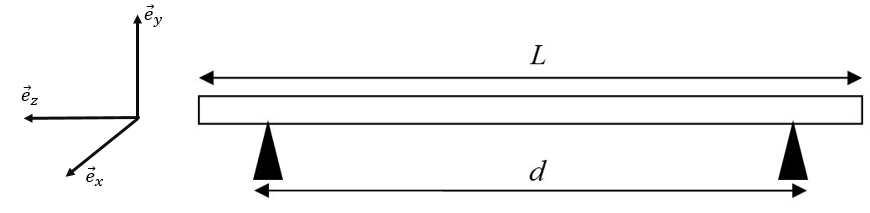
\includegraphics[scale=0.4]{Img_RDM_1.PNG}
\caption{Notations utilisées pour représenter la poutre à étudier.}
\label{Fig_RDM_Notations}
\end{figure}

Si nous chargeons la poutre d'une force $\vec{F}_1$ verticale, elle se déforme dans le plan vertical qui contient la poutre et la force (voir Fig.~\ref{Fig_RDM_Notations2}). Chaque point de la poutre décrit une trajectoire que l'on peut considérer comme verticale puis s'arrête en une position d'équilibre. Mesurons le déplacement d'un point $P$ et notons le $u_{1F}$. Enlevons la force $\vec{F}_1$  et exerçons une force $\vec{F}_2$.  Mesurons de nouveau le déplacement et notons le $u_{2F}$. Si nous exerçons maintenant simultanément $\vec{F}_1$  et $\vec{F}_2$ , nous constatons que la mesure du déplacement total vaut :
\begin{equation*}
u_F =u_{1F}+u_{2F}
\end{equation*}
C'est le théorème de superposition : l'application préalable d'une force $\vec{F}_1$  n'a pas d'influence sur le déplacement dû à $\vec{F}_2$.
\vspace{\baselineskip}

Si la poutre et les appuis ont, dans le plan vertical, le même axe de symétrie et que l'on applique une force suivant cet axe de symétrie ou des groupes de deux forces d'égale intensité symétriques par rapport à cet axe, la déformation est aussi symétrique par rapport à cet axe.
\vspace{\baselineskip}

Le déplacement d'un point s'appelle la flèche au point considéré. La flèche maximale s'appelle la flèche de la poutre. Si tout est symétrique par rapport à l'axe cité ci-dessus, cette flèche maximale se produit au milieu de la poutre. Dans les essais qui suivent, on appliquera la force au milieu de la poutre. Dans ce cas, la flèche au milieu de la poutre est donnée par la formule suivante :
\begin{equation}
u_F = \dfrac{Fd^3}{48 EI}
\end{equation}
avec $E$ le module d'Young et $I$ le moment d'inertie (ou moment quadratique).

\begin{figure}[h!]
\centering
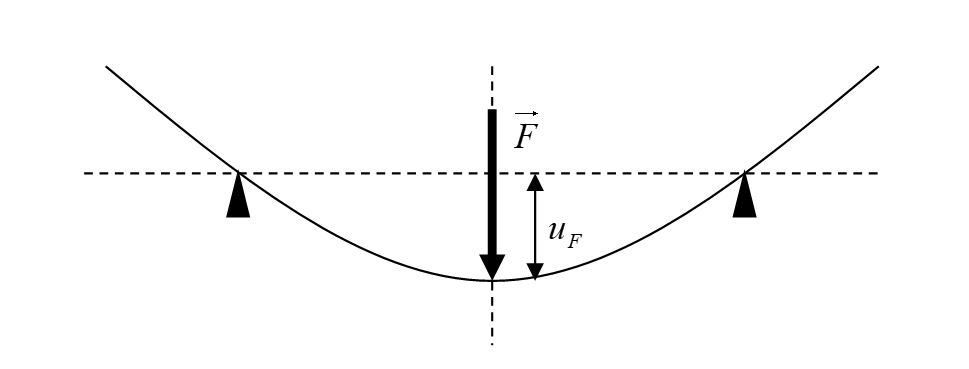
\includegraphics[scale=0.4]{Img_RDM_2.JPG}
\caption{Schématisation d'une poutre en flexion. Illustration des notations utilisées.}
\label{Fig_RDM_Notations2}
\end{figure}

Quand nous faisons varier la portée, une partie de la poutre, donc une partie de la charge due à la pesanteur, est à l'extérieur des appuis et cette partie est variable. Pour déterminer la flèche due aux seules forces, nous commencerons par déterminer la valeur de la flèche pour la poutre soumise à son poids propre plus le poids des outillages, puis pour la poutre lorsque les forces lui sont appliquées. C'est la différence de ces deux flèches, pour une même position des appuis, qui servira de base de calcul.


\paragraph*{Questions préliminaires à l'essai de flexion}
\begin{enumerate}
\item \ding{46} Calculer le moment d'inertie $I$ d'une poutre à section rectangulaire $\mathcal{S}$ par rapport à l'axe $Ox$. On notera $b$ (largeur) le côté suivant l'axe des $x$ et $h$ (épaisseur) le côté suivant l'axe $y$. On rappelle que :
\begin{equation}
I=I_x = \iint_{\mathcal{S}} y^2 dS
\end{equation}
\item \ding{46} Calculer le moment d'inertie $I$ d'une poutre à section circulaire $\mathcal{S}$ par rapport à l'axe $Ox$.
\end{enumerate}

\paragraph*{Relation entre portée et flèche}

\begin{description}
  \item[$\bullet$] \textbf{Mode opératoire.}
\begin{itemize}[label = \ding{110} , font =\tiny]
\item Posez la poutre à section rectangulaire en acier symétriquement sur des appuis distants de $300\, mm$ (on démontre que dans cette position la flèche est négligeable) ;
\item Posez l'équipage porte poids au milieu de la poutre ;
\item Amenez le comparateur de manière à placer sa touche au-dessus du milieu de la poutre ;
\item Descendez le comparateur jusqu'à ce que la grande aiguille ait fait quelques tours et calez-le ;
\item Tournez le cadran afin que la grande aiguille indique zéro.
\end{itemize}

  \item[$\bullet$] \textbf{Mesures et analyse.}
\begin{enumerate}[resume]
\item Pour une même masse placée sur le porte poids, relevez la flèche $u_F$ pour des portées $d$ de $300\, mm$, $400\, mm$, $500\, mm$ et $600\, mm$. On prendra bien soin entre chaque mesure de remettre le comparateur à zéro. Synthétiser vos résultats dans un tableau.
\item Faites un graphique en portant les flèches en ordonnée (échelle linéaire) et les portées en abscisses (échelle cubique). Que constatez-vous ?
\item Déterminez le module d'Young du matériau. Expliquez clairement votre démarche.
\end{enumerate}

\end{description}

\paragraph*{Relation entre flèche et force appliquée (charge)}

\begin{description}
  \item[$\bullet$] \textbf{Mode opératoire.}
\begin{itemize}[label = \ding{110} , font =\tiny]
\item Posez une éprouvette sur des appuis distants de $d=600\, mm$ ;
\item Placez le dispositif de mise en charge au centre de la poutre et réglez le comparateur sur le zéro ;
\item Appliquez successivement des charges de $5$, $10$, $15$ et $20\, N$ et faites les lectures des déplacements correspondants.
\end{itemize}

\item[$\bullet$] \textbf{Mesures et analyse.}
\begin{enumerate}[resume]
\item Consignez les résultats dans un tableau et faire un graphique. Commenter les résultats obtenus.
\item Déterminez le module d'Young du matériau.
\end{enumerate}

\end{description}

\paragraph*{Relation entre flèche et largeur}

\begin{description}

\item[$\bullet$] \textbf{Mode opératoire.} Pour cette expérience, vous veillerez à utiliser les poutres ayant une même hauteur.
\begin{itemize}[label = \ding{110} , font =\tiny]
\item Placez les appuis à $500\, mm$ l'un de l'autre et poser une poutre ;
\item Chargez cette poutre avec un poids de $5\, N$ en son centre ;
\item Prenez les poutres ayant une même hauteur mais des largeurs différentes et refaites la même mesure avec chacune de ces poutres.
\end{itemize}

\item[$\bullet$] \textbf{Mesures et analyse.}
\begin{enumerate}[resume]
\item Consignez les résultats des flèches mesurées dans un tableau.
\item Tracez un graphique avec les résultats en plaçant en ordonnées les valeurs de flèche mesurée et en abscisses le terme $\dfrac{1}{b}$.  Commentez le graphique obtenu.
\item Calculez le module d'Young du matériau.
\end{enumerate}

\end{description}

\paragraph*{Relation entre flèche et épaisseur}
Le principe de la mesure ne change pas si ce n'est que cette fois-ci seule l'épaisseur de l'éprouvette varie.
\begin{enumerate}[resume]
\item Consignez les résultats des flèches mesurées pour chaque éprouvette (même largeur et épaisseur variable) dans un tableau.
\item Tracez un graphique avec les résultats en plaçant en ordonnées les valeurs de flèche mesurée et en abscisses le terme $1/h^3$ .  Que constatez-vous ?
\item Calculez le module d'Young du matériau.
\end{enumerate}

\paragraph*{Détermination du module d'Young pour les éprouvettes cylindriques}
\begin{enumerate}[resume]
\item Pour trois des éprouvettes cylindriques disponibles (acier, laiton, aluminium et cuivre), tracez la flèche $u_F$ en fonction de la charge $F$.
\item Calculez les modules d'Young des matériaux étudiés.
\item Comparez les valeurs expérimentales obtenues avec les valeurs de la littérature. On calculera les écarts relatifs. On donne les modules d'Young du cuivre $E=124\,GPa$, du laiton $E=100\,GPa$, de l'acier $E=203\, GPa$ et de l'aluminium $E=69\,GPa$.
\end{enumerate}

%
%\subsection{Essais de torsion}
%\subsubsection{Rappel théorique}
%On dit qu'une poutre est soumise à une torsion quand elle est soumise à un couple autour de son axe longitudinal. La torsion est dite pure si le couple agit seul.
%
%Pour réaliser cette situation, on place les deux extrémités de la poutre dans deux appuis. L'une des extrémités est bloquée et l'autre peut tourner uniquement autour de l'axe mentionné ci-dessus si on y applique un couple. Juste après l'articulation, on bloque un levier autour de la poutre (voir Fig.~\ref{Fig_RDM_montage}). À l'autre extrémité de ce levier, on applique différentes forces $\vec{P}$.
%
%\begin{minipage}{\textwidth}
%\begin{minipage}{0.45\textwidth}
%\begin{figure}[H]
%\centering  \includegraphics[scale=0.4]{Img_Torsion}
%\caption{Représentation schématique pour le montage de torsion.}
%\label{Fig_RDM_montage}
%\end{figure}
%\end{minipage} \hspace{0.5cm}
%\begin{minipage}{0.45\textwidth}
%\begin{figure}[H]
%\centering \includegraphics[scale=0.4]{Img_contrainte}
%\caption{Contraintes tangentielles dans une poutre en torsion.}
%\label{Fig_RDM_tau}
%\end{figure}
%\end{minipage}
%\end{minipage}
%\vspace{\baselineskip}
%
%La réaction verticale de l'appui $\vec{F}$ forme avec $\vec{P}$ un couple qui agit sur la poutre. La résistance à la torsion provient de ce qu'une section transversale agit sur la section infiniment voisine en glissement, comme pour la traction. Les contraintes sont donc dans les plans transversaux de la poutre : on les appelle contraintes de cisaillement ou contraintes tangentielles et on les note $\tau$. Dans la torsion pure, ces contraintes sont symétriques par rapport à l'axe de la pièce comme on peut le constater Fig.~\ref{Fig_RDM_tau}.
%
%
%L'extrémité sollicitée, ou toute section transversale de la poutre, subit autour de l'axe une rotation dont l'amplitude est donnée par :
%\begin{equation}
%\theta = \dfrac{C l}{I_p G}
%\end{equation}
%avec $C$ le moment de torsion, $l$ la longueur de la poutre à partir de l'extrémité fixe, $I_p$ le moment d'inertie polaire et $G$ le module de cisaillement.
%
%
%\paragraph*{Contrainte tangentielle maximale $\tau_{max}$.} La tension tangentielle ou contrainte tangentielle maximale $\tau_{max}$ est donnée par la formule :
%\begin{equation}
%\tau_{max} = \dfrac{C D}{2I_p}
%\end{equation}
%avec $D$ le diamètre de la poutre.
%
%\paragraph*{Moment de torsion $C$.} Dans la sollicitation présente, le moment de torsion $C$ est donné par :
%\begin{equation}
%C = Fd
%\end{equation}
%où $d$ correspond à la distance du bras de levier. Ici $d=100\,mm$.
%
%
%\paragraph*{Angle de torsion $\theta$.} L'angle de torsion est obtenu à partir de la valeur de la longueur $L$ qui est lue au comparateur après application des forces. Plus précisément, on montre que l'angle de torsion est donné par la relation suivante :
%\begin{equation}
%\theta = \arctan \left( \dfrac{L}{\dfrac{d}{2}} \right) \approx \dfrac{2L}{d}
%\end{equation}
%où la mesure de la longueur $L$ se fait à la moitié du bras de levier.

%
%\subsubsection{Questions préliminaires à l'essai de torsion}
%\begin{enumerate}[resume]
%\item Exprimer en fonction du diamètre $D$ de la poutre le moment d'inertie polaire $I_p$ de la section $\mathcal{S}$ défini par  :
%\begin{equation}
%I_p = \iint_{\mathcal{S}} r^2 dS
%\end{equation}
%\item Faire l'application numérique.
%\item En réalisant une analyse dimensionnelle, donner les dimensions du module de cisaillement $G$ et de la contrainte tangentielle $\tau$. On utilisera les millimètres ($mm$) comme unité de longueur ainsi que le Newton ($N$).
%\end{enumerate}
%
%\subsubsection{Manipulations}
%\paragraph*{Mode opératoire.}
%\begin{itemize}[label = \ding{110}, font = \tiny]
%\item 	Réglez les supports à $600\, mm$ ;
%\item Desserrez les vis de blocage dans les supports à l'aide des clés Allen ;
%\item Introduisez la poutre d'essai ;
%\item Resserrez les vis de blocage du côté fixe ;
%\item Placez horizontalement le levier du dispositif de torsion et serrez les vis de blocage ;
%\item Placez l'équipage porte poids à l'extrémité ;
%\item Amenez le comparateur et descendez sa touche sur le centre de l'équipage. \item Continuez à descendre jusqu'à ce que la grande aiguille ait fait quelques tours ;
%\item Tournez le cadran du comparateur jusqu'à ce que la lecture à la grande aiguille soit zéro.
%\end{itemize}
%
%\paragraph*{Mesures et analyse.}
%\begin{enumerate}[resume]
%\item Pour une poutre cylindrique de votre choix, exercez successivement des forces de $5$, $10$ et $15\, N$ et relevez, dans un tableau, les déplacements mesurés.
%\item Dans le même tableau, calculez le moment de torsion $C$, la contrainte de cisaillement maximale $\tau_{max}$ l'angle de torsion $\theta$ (en radian) et le module de cisaillement $G$.
%\end{enumerate}


\end{document}
